% vim:tw=0
% vim:fdm=syntax
\documentclass[a4paper,12pt]{scrartcl}
\usepackage{mythesis}
%
\author{Sakari Cajanus}
\studentnumber{82036R}
\email{sakari.cajanus@aalto.fi}

\title{Exercise Round 1}{Och samma på English}
\place{Espoo}
\thesisdegree{S-114.1100 Computational Science}{Bachelor's Thesis}
%\instructor{FT Mari Myllymäki}{Ph.D. Mari Myllymäki}
%\supervisor{TkT Markus Turunen}{D.Sc. (Tech.) Markus Turunen}

\uni{Aalto-yliopisto}{Aalto University}
\school{sähkötekniikan korkeakoulu}{School of Electrical Engineering}
\degreeprogram{Bioinformaatioteknologia}{Bioinformation technology}
\department{Lääketieteellisen tekniikan ja laskennallisen tieteen laitos}{Department of Biomedical Engineering and Excellence in Computational Science}
\keywords{suomeksi}{englanniksi}

\hypersetup{%
    colorlinks=true, linktocpage=false, pdfstartpage=1, pdfstartview=FitV,%
    % uncomment the following line if you want to have black links (e.g., for printing)
    %colorlinks=false, linktocpage=false, pdfborder={0 0 0}, pdfstartpage=3, pdfstartview=FitV,% 
    breaklinks=true, pdfpagemode=UseNone, pageanchor=true, pdfpagemode=UseOutlines,%
    plainpages=false, bookmarksnumbered, bookmarksopen=true, bookmarksopenlevel=1,%
    hypertexnames=true, pdfhighlight=/O,%hyperfootnotes=true,%nesting=true,%frenchlinks,%
    urlcolor=blue, linkcolor=blue, citecolor=green, %pagecolor=RoyalBlue,%
    %urlcolor=Black, linkcolor=Black, citecolor=Black, %pagecolor=Black,%
    pdftitle={\thetitle},%the title
    pdfauthor={\theauthor},%your name
    pdfsubject={\thetitle},%
    pdfkeywords={\thekeywords},%
    pdfcreator={XeLaTeX},%
    pdfproducer={A happy XeLaTeX user}%
}

\begin{document}
%\pagenumbering{roman}
\maketitlepage
\clearpage
\pagenumbering{arabic}
\section{Plots and conclusions}
The function
\begin{align*}
\hspace{-10mm}(a)\hspace{10mm}f_1(x)=\frac{e^x -1}{x}
\end{align*}
has potential loss of significance near $x=0$. This is because the exponential function $e^x$ has limit
\begin{align*}
\lim_{x\to0}e^x=1
\end{align*}
and we end up substracting almost equal values. The error is further amplified by the division by small $x$. For example, when $x=1\times10^{-3}$ 
\begin{align*}
e^x=1.001000500166708...
\end{align*}
Now we have from the substraction $e^x-1$
\begin{align*}
1-\frac{1}{e^x}=0.000999500166625...
\end{align*}
This lies between values $2^{-9}=0.001953125$ and $2^{-10}=0.0009765625$ so at least 9 but at most 10 bits are lost. It is also worth pointing out that for $x$ near zero, the series expansion
\begin{align*}
\frac{e^x-1}{x}=1 + \frac{x}{2!} + \frac{x^2}{3!} + \frac{x^3}{4!} + \ldots
\end{align*}
converges to $1$ quite rapidly: to avoid loss of significance, this is what we should use.
\begin{figure}[h!]
  \centering
    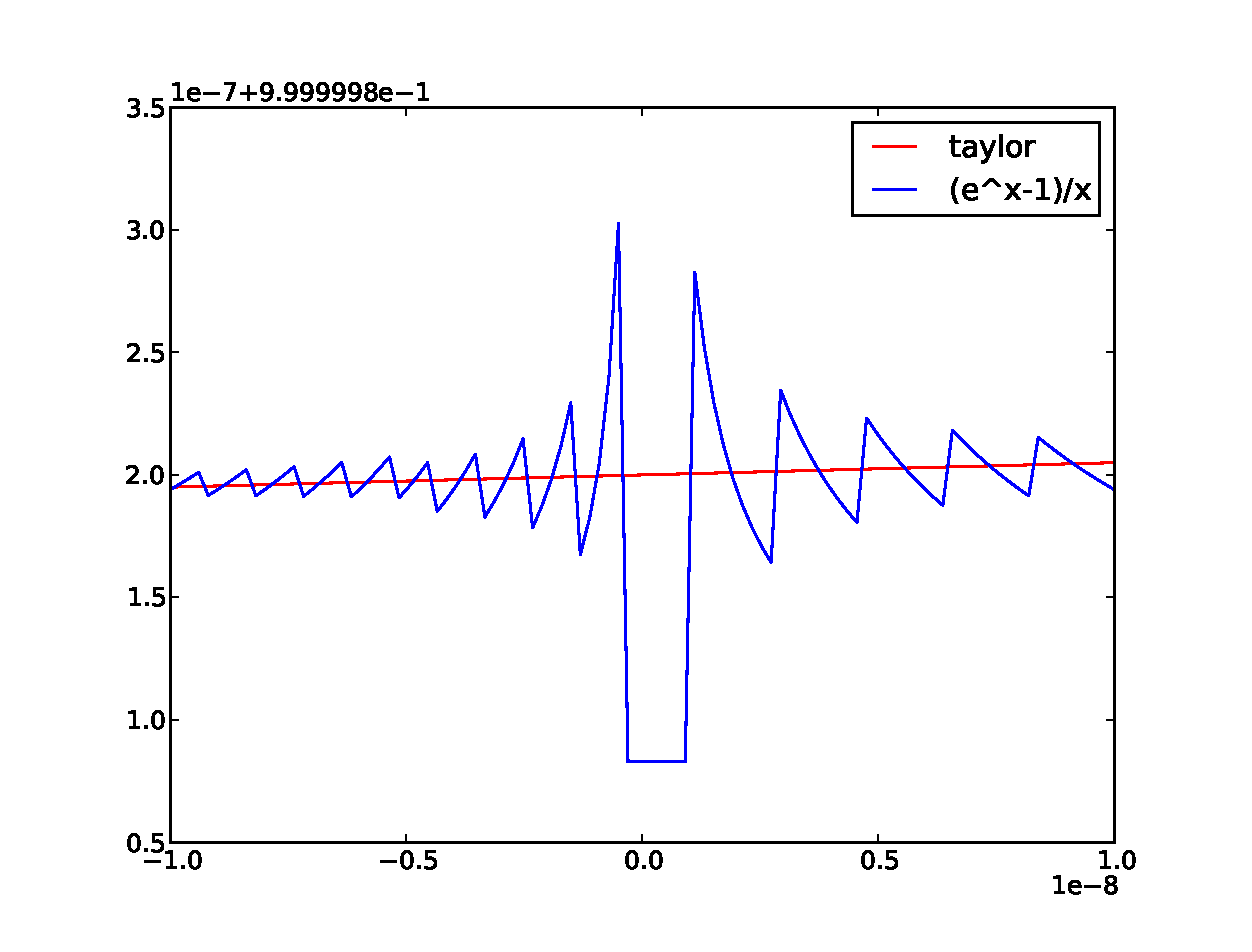
\includegraphics[width=0.7\textwidth]{taylor}
  \caption{Approximation by 4th degree Taylor polynomial and function itself.}
  \label{fig:taylor}
\end{figure}
In Figure \ref{fig:taylor} you can see both the Taylor approximation $(n=4)$ and function values with the values calculated in 100 points between $x=-1\times10^{-9}$ and $x=1\times10^{-9}$. The behaviour of the function when the approximation is not used is heavily dependant on which points it's values are calculated: If we'd choose different number of points or different interval, the function would look quite different.


Estimate of the error of the Taylor approximation is given by the $(n+1)$th term in the series. In this case, for $x=1\times10^{-9}$, it is
\begin{align*}
R(n+1)=\frac{x^4}{5!}=8.333\ldots\times10^{-39}.
\end{align*}
It is also worth mentioning that python has built-in function \emph{expm1(x)} that is meant to be used for calculating $e^x-1$ when $x<\log 2$.

With the function
\begin{align*}
\hspace{-10mm}(b)\hspace{10mm}f_2(x)=\frac{e^x - e^{-x}}{2x}
\end{align*}
we face the similar problem. Both terms in the numerator converge to one as $x$ approaches zero:
\begin{align*}
\lim_{x\to0}e^x=1\\
\lim_{x\to0}e^{-x}=1
\end{align*}
As before, we can write the function as a series expansion
\begin{align*}
\frac{e^x - e^{-x}}{2x}=1 + \frac{x^2}{3!} + \frac{x^4}{5!} + \frac{x^6}{7!} + \ldots
\end{align*}
Using just the first two terms $(n=4)$, as before, we get following figure \ref{fig:taylor2} as $x$ get values between $x=-1\times10^{-6}$ and $x=-1\times10^{-6}$.
\begin{figure}[h!]
  \centering
    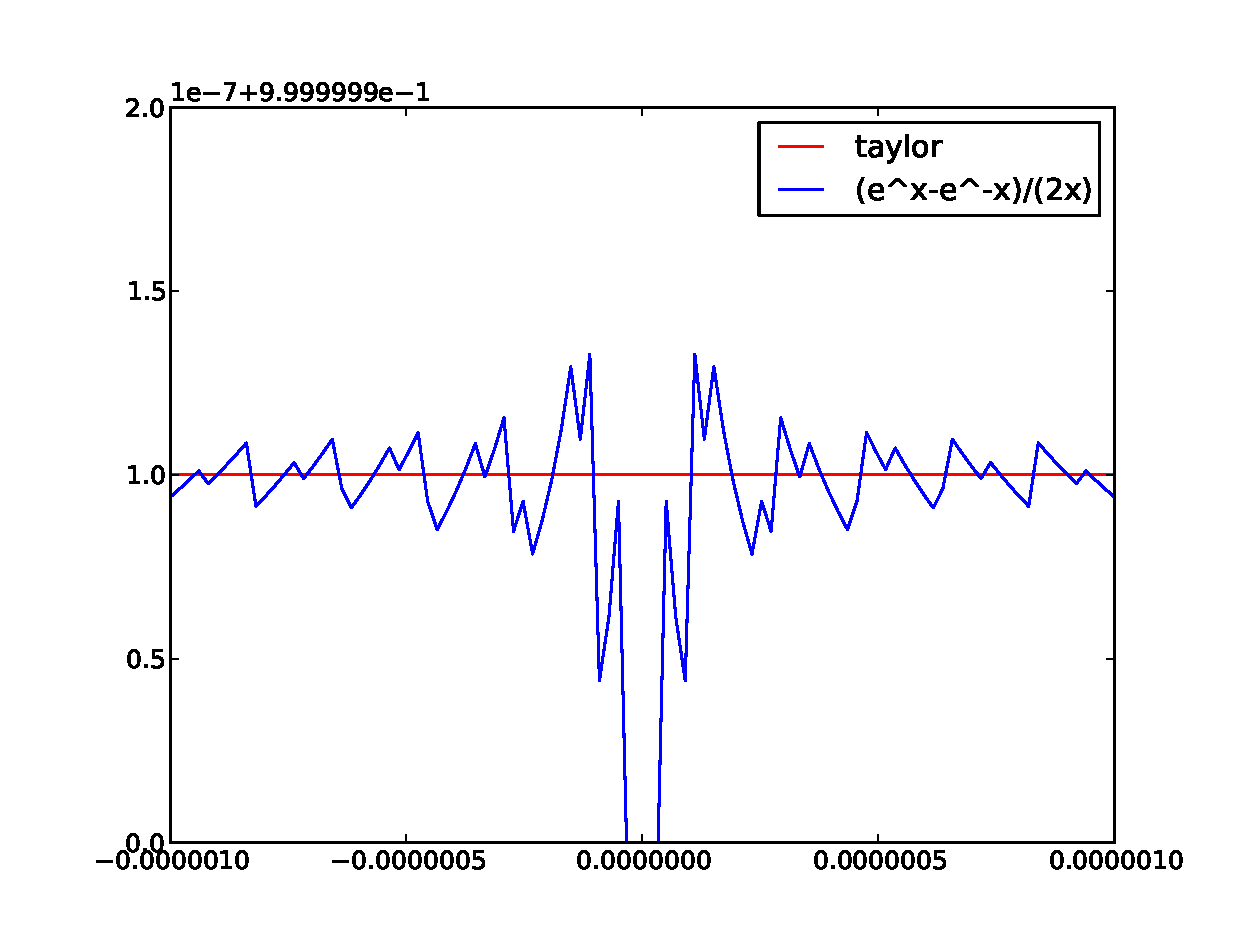
\includegraphics[width=0.7\textwidth]{taylor2}
  \caption{Approximation by 4th degree Taylor polynomial and function itself.}
  \label{fig:taylor2}
\end{figure}

We can calculate the error estimate of the approximation at $x=1\times10^{-6}$ using the next term in series
\begin{align*}
R(n+1)=\frac{x^4}{5!}=8.333\ldots\times10^{-27}.
\end{align*}

\clearpage
\section{Plots and conclusions}
\begin{verbatim}
i                   x                    f(x)
0            0.577350                -5.384900
1     -5774691.304827 -192568975495066910720.0
2     -3849794.203218  -57057474220760129536.0
3     -2566529.468812  -16905918287632351232.0
4     -1711019.645875   -5009160974113097728.0
5     -1140679.763917   -1484195844181532416.0
                   ...
44          -1.762824                -8.715240
45          -0.715653                -4.650875
46           7.953624               490.193685
47           5.356989               143.374340
48           3.672056                40.841946
49           2.636825                10.696613
50           2.098184                 2.138817
\end{verbatim}
As a result of very bad starting point choice, the first calculated values of the iteration for both $x$ and the function value $f(x)$ are very small. This is a result of the derivate being close to zero, $-9.32499999884\times10^{-07}$. In fact, 50 steps are not sufficient to get to the root after this detour. Function $x^3-x-5$ and its tangent at start point are shown in Figure \ref{fig:newton}.
\begin{figure}[h!]
  \centering
    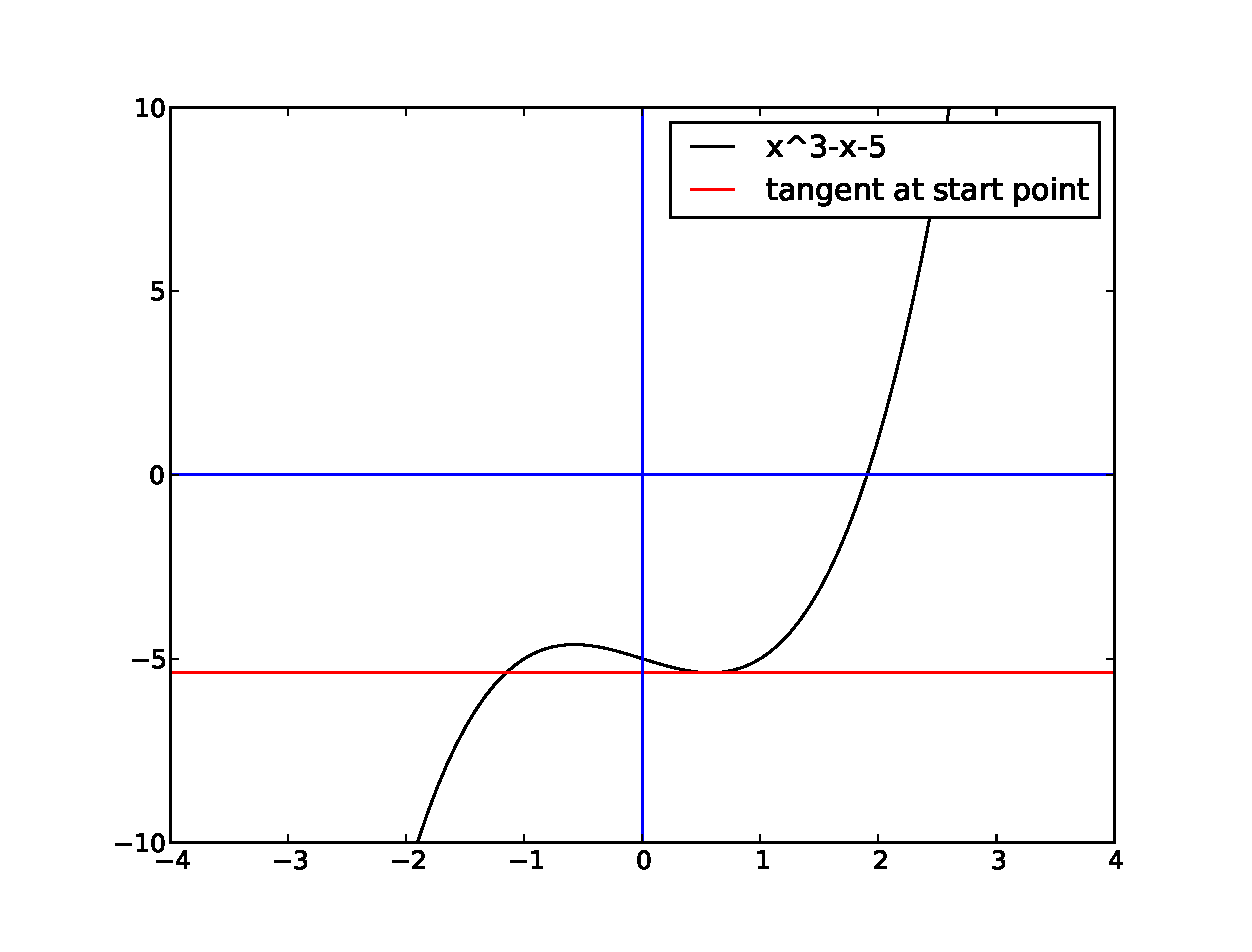
\includegraphics[width=0.7\textwidth]{newton}
  \caption{function $x^3-x-5$ and our very bad starting point choice.}
  \label{fig:newton}
\end{figure}
Learning from this, we improve our algorithm by making it use bisection method if the new $x$ value calculated with Newton's method would take us out of certain bounds, where the root is known to reside. In this case, bounds $a=0$ and $b=3$ were used. Here is the output:
\begin{verbatim}
i                   x                f(x)
0            0.577350           -5.384900
1            1.500000           -5.000000
2            2.369565            5.935163
3            1.994977            0.944903
4            1.908605            0.044005
5            1.904172            0.000112
6            1.904161            0.000000
Found root at 1.904161
\end{verbatim}
Nice and quick!
\clearpage
\section{Plots and conclusions}
In problem 3 we were asked to examine basins of attraction of three roots in complex plane. The complex polynomial
\begin{align*}
z^3-1
\end{align*}
has three roots:
\begin{align*}
z&=1\\
z&\approx-0.5 + 0.866025i\\
z&\approx-0.5 - 0.866025i.
\end{align*}
These three roots were assigned a different color, and pixels in a $1000\times1000$ square containing region $-1\le\text{Real}(z)\le 1$ and $-1\le\text{Imag}(z)\le 1$ were assigned this same color if the function starting from the point would reach the root in 100 iterations. Figure \ref{fig:fractal} shows the results.
\begin{figure}[h!]
  \centering
    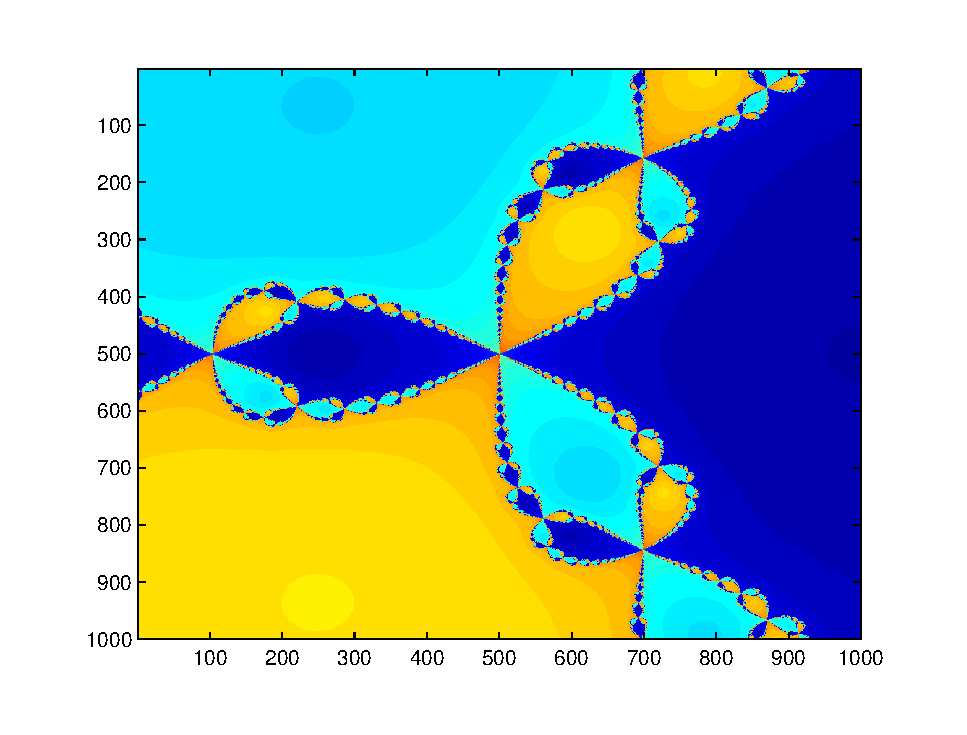
\includegraphics[width=0.7\textwidth]{fractal}
  \caption{Three basins of attraction featuring ugly colors.}
  \label{fig:fractal}
\end{figure}
\clearpage

\appendix
\lstset{basicstyle=\ttfamily, numbers=left, numberstyle=\tiny, stepnumber=1, numbersep=5pt}
\gdef\thesection{Appendix \arabic{section}.}
\clearpage

\section{Code\label{LiiteA}}
\lstinputlisting[language=Python]{ex1_prob1_f.py}
\clearpage
\section{Code\label{LiiteB}}
\subsection{Only Newton}
\lstinputlisting[language=C]{ex1_prob2.c}
\clearpage
\subsection{A (hacky) solution using Newton/bisection hybrid method}
\lstinputlisting[language=C]{ex1_prob2_hybrid.c}
\clearpage
\section{Code\label{LiiteC}}
\lstinputlisting[language=matlab]{matlab_fractal.m}
\end{document}
